%!TEX root=../../main.tex

\chapter{Simple linear regression}
\label{linRegrForTwoVar}

\begin{comment}
  
  - indexing not done yet
  - exercise file not done yet
\end{comment}


\index{linear regression|textbf}

The relationship between two numerical variables can be visualized using a scatterplot in the $xy$-plane. The \term{predictor} or \term{explanatory variable} is plotted on the horizontal axis, while the \term{response variable} is plotted on the vertical axis.\footnote{Sometimes, the predictor variable is referred to as the independent variable, and the response variable referred to as the dependent variable.} 

This chapter explores simple linear regression, a technique for estimating a straight line that best fits data on a scatterplot. A line of best fit functions as a linear model that can not only be used for prediction, but also for inference. Linear regression should only be used with data that exhibit linear or approximately linear relationships. 

For example, scatterplots in Chapter~\ref{introductionToData} illustrated the linear relationship between height and weight in the NHANES data, with height as a predictor of weight. Adding a best-fitting line to these data using regression techniques would allow for prediction of an individual's weight based on their height. The linear model could also be used to investigate questions about the population-level relationship between height and weight, since the data are a random sample from the population of adults in the United States. 

The next chapter covers multiple regression, a statistical model used to estimate the relationship between a single response variable and several predictor variables.

\section{Examining scatterplots}
\label{examiningScatterPlots}

\index{scatterplots|(}
Various demographic and cardiovascular risk factors were collected as a part of the Prevention of REnal and Vascular END-stage Disease (PREVEND) study, which took place in the Netherlands. The initial study population began as 8,592 participants aged 28-75 years who took a first survey in 1997-1998.\footnote{Participants were selected from the city of Groningen on the basis of their urinary albumin excretion; urinary albumin excretion is known to be associated with abnormalities in renal function.} Participants were followed over time; 6,894 participants took a second survey in 2001-2003, and 5,862 completed the third survey in 2003-2006. In the third survey, measurement of cognitive function was added to the study protocol. Data from 4,095 individuals who completed cognitive testing are in the \data{prevend} dataset, available in the \textsf{R} \texttt{oibiostat} package. 

As adults age, cognitive function changes over time, largely due to various cerebrovascular and neurodegenerative changes. It is thought that cognitive decline is a long-term process that may start as early as 45 years of age.\footnote{Joosten H, et al. Cardiovascular risk profile and cognitive function in young, middle-aged, and elderly subjects. Stroke. 2013;44:1543-1549, \url{https://doi.org/10.1161/STROKEAHA.111.000496} } The Ruff Figural Fluency Test (RFFT) is one measure of cognitive function that provides information about various cognitive abilities such as planning and the ability to switch between different tasks. The test consists of drawing as many unique designs as possible from a pattern of dots, under timed conditions; scores range from 0 to 175 points (worst and best score, respectively).

RFFT scores for a random sample of 500 individuals are shown in Figure~\ref{prevendAgeRFFT}, plotted against age at enrollment, which is measured in years. The variables \var{Age} and \var{RFFT} are negatively associated; older participants tend to have lower cognitive function. There is an approximately linear trend observable in the data, which suggests that adding a line could be useful for summarizing the relationship between the two variables.

\begin{figure}[h!]
	\centering
	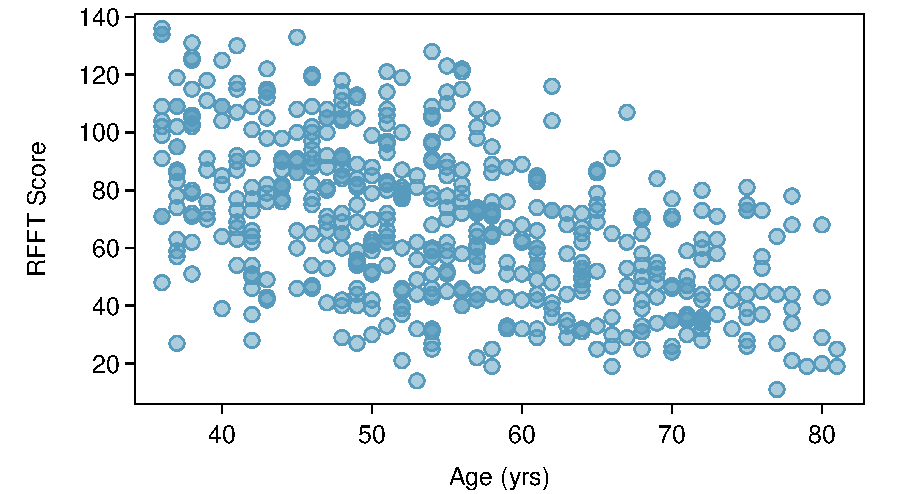
\includegraphics[width=0.8\textwidth]
	{ch_simple_linear_regression_oi_biostat/figures/prevendAgeRFFTPlot/prevendAgeRFFTPlot}
	\caption{A scatterplot showing \var{age} vs. \var{RFFT}. Age is the predictor variable, while RFFT score is the response variable.}
	\label{prevendAgeRFFT}
\end{figure}

It is important to avoid adding straight lines to non-linear data. For example, the scatterplot in Figure~\ref{incomeLifeExpectancy} of Chapter~\ref{introductionToData} shows a highly non-linear relationship between between annual per capita income and life expectancy for 248 countries in 2012.

The following conditions should be true in a scatterplot for a line to be considered a reasonable approximation to the relationship in the plot and for the methods of inference discussed later in the chapter:


\index{linear regression ! assumptions}


\begin{description}
\setlength{\itemsep}{0mm}
\item[1 Linearity.] The data shows a linear trend. If there is a nonlinear trend, an advanced regression method should be applied; such methods are not covered in this text.  Occasionally, a transformation of the data will uncover a linear relationship in the transformed scale.
\item[2 Constant variability.] The variability of the response variable about the line remains roughly constant as the predictor variable changes.
\item[3 Independent observations.]  The $(x,y)$ pairs are independent; i.e., the value of one pair provides no information about other pairs. Be cautious about applying regression to sequential observations in time (\term{time series} data), such as height measurements taken over the course of several years. Time series data may have a complex underlying structure, and the relationship between the observations should be accounted for in a model. 
\item[4 Residuals that are approximately normally distributed.] This condition can be checked only after a line has been fit to the data and will be explained in Section~\ref{checkingResiduals}. In large datasets, it is sufficient for the residuals to be approximately symmetric with only a few outliers. This condition becomes particularly important when the inferences are made about the line, as discussed in Section~\ref{inferenceRegression}.  
\end{description}

\begin{exercise} \label{nonConstantVariance}
Figure~\ref{frogClutchVolBodySizeRegress} shows the relationship between \var{clutch.volume} and \var{body.size} in the \data{frog} data.  The plot also appears as Figure~\ref{frogClutchVolBodySize} in Chapter~\ref{introductionToData}. Are the first three conditions met for linear regression?\footnote{No. While the relationship appears linear and the observations are independent, the variability in \var{clutch.volume} is noticeably less for small values of \var{body.size} than for larger values of \var{body.size}.}

\begin{figure}[h!]
	\centering
	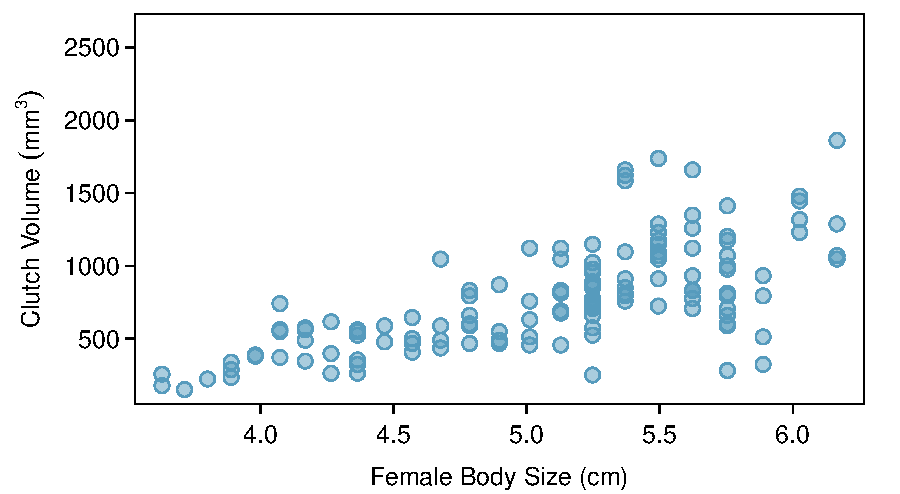
\includegraphics[width=0.6\textwidth]
	{ch_intro_to_data_oi_biostat/figures/frogClutchVolBodySize/frogClutchVolBodySize}
	\caption{A plot of \var{clutch.volume} versus \var{body.size} in the \data{frog} data.}
	\label{frogClutchVolBodySizeRegress}
\end{figure}


\end{exercise}

\index{scatter plots|)}
\section{Estimating a regression line using least squares}
\label{estimatingLeastSquaresLine}

\index{least squares regression |(}

Figure~\ref{prevendResid} shows the scatterplot of age versus RFFT score, with the \term{least squares regression line} added to the plot; this line can also be referred to as a \term{linear model} for the data. An RFFT score can be predicted for a given age from the equation of the regression line:

\[\widehat{\text{RFFT}} = 137.55 - 1.26(\text{age}). \]


The vertical distance between a point in the scatterplot and the predicted value on the regression line is the \term{residual} for the point; observations below the line have negative residuals, while observations above the line have positive residuals. The size of a residual is usually discussed in terms of its absolute value; for example, a residual of -13 is considered larger than a residual of 5 since $|-13| = 13 > 5$.

For example, consider the predicted RFFT score for an individual of age 56. According to the linear model, this individual has a predicted score of $137.550 - 1.261(56) = 66.934$ points. In the data, however, there is a participant of age 56 with an RFFT score of 72; their score is about 5 points higher than predicted by the model (the residual for this observation is shown on the plot with a ``$\times$'').

\begin{figure}[h!]
	\centering
	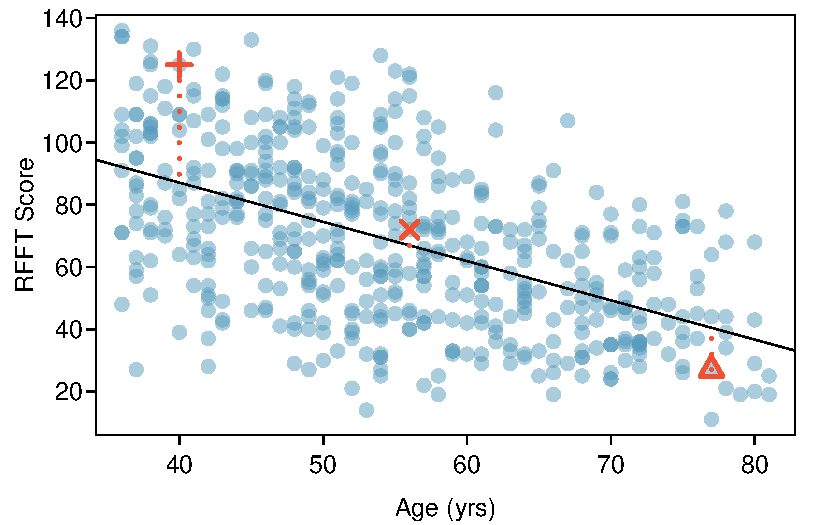
\includegraphics[width=0.8\textwidth]
	{ch_simple_linear_regression_oi_biostat/figures/prevendResid/prevendResid.pdf}
	\caption{A scatterplot showing \var{age} (horizontal axis) vs. \var{RFFT} (vertical axis) with the regression line added to the plot. Three observations are marked in the figure; the one marked by a ``$+$'' has a large residual of about +38, the one marked by a ``$\times$'' has a small residual of about +5, and the one marked by a ``$\triangle$'' has a moderate residual of about -13.}
	\label{prevendResid}
\end{figure}

\begin{termBox}{\tBoxTitle{Residual: difference between observed and expected}
The residual of the $i^{th}$ observation $(x_i, y_i)$ is the difference of the observed response ($y_i$) and the response predicted based on the model fit ($\widehat{y}_i$):
\begin{eqnarray*}
e_i = y_i - \widehat{y}_i
\end{eqnarray*}
The value $\widehat{y}_i$ is calculated by plugging $x_i$ into the model.}
\end{termBox}

The \term{least squares regression line} is the line which minimizes the sum of the squared residuals for all the points in the plot.  Let $\hat{y}_i$ be the predicted value for an observation with value $x_i$ for the explanatory variable.  The value $e_i = y_i - \hat{y}_i$ is the residual for a data point $(x_i, y_i)$ in a scatterplot with $n$ pairs of points.  The least squares line is the line for which
\begin{eqnarray}
e_{1}^2 + e_{2}^2 + \dots + e_{n}^2
\label{sumOfSquaresForResiduals}
\end{eqnarray}
is smallest.


For a general population of ordered pairs $(x,y)$, a \term{population regression model} is written 
\begin{align*}
	 y = \beta_0 + \beta_1x + \varepsilon.
\end{align*}
The term $\varepsilon$ is a normally distributed `error term' that has mean 0 and standard deviation $\sigma$. Since $E(\varepsilon) = 0$,  the model can also be written
\begin{align*}
	E(Y|x) = \beta_0 + \beta_1 x,
\end{align*}
where the notation $E(Y|x)$ denotes the expected value of $Y$ when the predictor variable has value $x$. 

For the PREVEND data, the population regression line can be written as
\begin{align*}
  \text{RFFT} &= \beta_0 + \beta_{1}\times \text{age} + \varepsilon, \, \text{or}
 E (\text{RFFT}| age) &= \beta_0 + \beta_{1}\times \text{age}.
\end{align*}
The term $\beta_0$ is the vertical intercept for the line (often referred to as simply the intercept) and $\beta_1$ is the slope.  These two values are called the \emph{parameters} of the line.  In statistical terms, the equation is called a population model for the regression, where specific values of the slope and intercept are estimated from the data. The notation $b_0$ and $b_1$ are used to represent the point estimates of the parameters $\beta_0$ and $\beta_1$.

\marginpar[\raggedright\vspace{0.5mm}

$b_0, b_1$\vspace{0.5mm}\\\footnotesize Sample\\estimates\\ of $\beta_0$, $\beta_1$]{\raggedright\vspace{0.5mm}
	
$b_0, b_1$\vspace{0.5mm}\\\footnotesize Sample\\estimates\\ of $\beta_0$, $\beta_1$}

\begin{itemize}
\item The slope of the least squares line is estimated by
\begin{eqnarray}
b_1 = \frac{s_y}{s_x} r,
\label{slopeOfLSRLine}
\end{eqnarray}
where $r$ is the correlation between the two variables, and $s_x$ and $s_y$ are the sample standard deviations of the explanatory variable and response, respectively.
\item The intercept for the regression line is estimated by
\begin{eqnarray}
b_0 = \overline{y} - b_1\overline{x}.
\label{interceptOfLSRLine}
\end{eqnarray}
\end{itemize}

\begin{example}{From the summary statistics displayed in Table~\ref{summaryAgeRFFT}, calculate the equation of the least-squares regression line for the PREVEND data.
		
\begin{table}[ht]
	\centering
	\begin{tabular}{l rr}
		\hline
		\vspace{-4mm} & & \\
		\vspace{0.4mm}	&	\ \ Age (yrs) (``$x$'')	& \ \ RFFT score (``$y$'') \\
		\hline
		\vspace{-3.9mm} & & \\
		mean	& $\overline{x} = 54.82$		& $\overline{y} = 68.40$ \\
		standard deviation		& $s_x = 11.60$		& $s_y = 27.40$\vspace{0.4mm} \\
		\hline
		\vspace{-4mm}\ &\\
		& \multicolumn{2}{r}{$r=-0.534$} \\
		\hline
	\end{tabular}
	\caption{Summary statistics for \var{age} and \var{RFFT} from a sample of the PREVEND data.}
	\label{summaryAgeRFFT}
\end{table}
}
	
\[b_1 = \frac{s_y}{s_x} r = \frac{27.40}{11.60}(-0.534) = -1.26\]

\[b_0 = \overline{y} - b_1\overline{x} = 68.40 - (5.14)(54.82) = 137.55. \]

The estimated line predicting RFFT score from age in these data is the one shown at the beginning of this section:
\begin{eqnarray*}
	\widehat{\text{RFFT}} = 137.55 - 1.26(\text{age}).
\end{eqnarray*}
	
\end{example}


\begin{exercise}
Figure~\ref{famussHeightWeightRegress} shows the relationship between \var{height} and \var{weight} in the FAMuSS dataset introduced in Chapter~\ref{introductionToData}. Calculate the equation of the regression line given the summary statistics: $\overline{x} = 66.83, \overline{y} = 155.65, s_{x} = 3.57, s_{y} = 34.59, r = 0.531$.\footnote{The equation of the line is $\widehat{weight} = -187.79 + 5.14(height)$, where height is in inches and weight is in pounds.}

\begin{figure}[h!] 
	\centering
	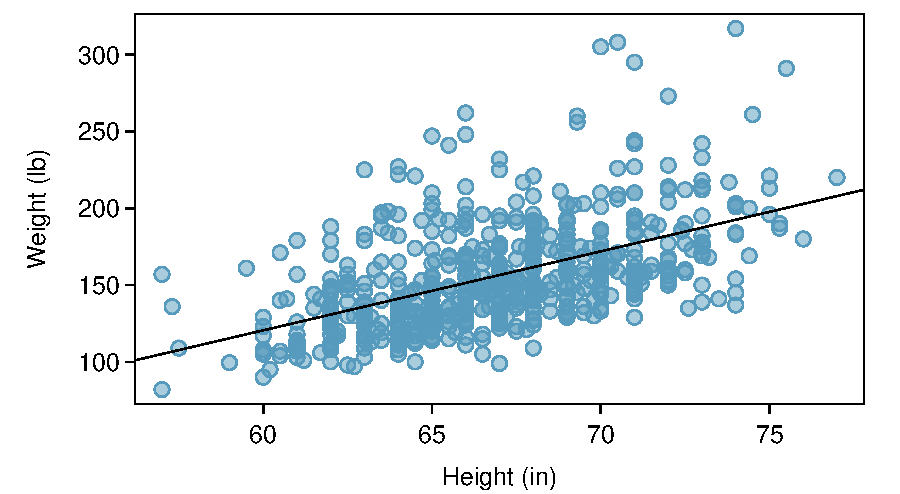
\includegraphics[width=0.6\textwidth]
	{ch_simple_linear_regression_oi_biostat/figures/famussHeightWeightRegress/famussHeightWeightRegress}
	\caption{A plot of \var{height} versus \var{weight} in the FAMuSS dataset, with a least-squares regression line}
	\label{famussHeightWeightRegress}
\end{figure}

	
\end{exercise}

\begin{exercise} \label{predictingFamussWeightfrmHeightMetric}
Predict the weight in kilograms for a FAMuSS participant who is 1.75 meters tall. 1 m = 39.37 in; 1 lb = 0.454 kg.\footnote{1.75 meters equals $(1.75)(39.37) = 68.90$ inches. From the regression equation, the predicted weight is $-187.79 + 5.14(68.90) = 166.36$ pounds. In kilograms, this weight is $(166.36)(0.454) = 75.53$.}
\end{exercise}

%\newpage

Typically, regression lines are estimated using statistical software, such as the statistical computing language \textsf{R}. The \textsf{R} companion to this text provides details on fitting a least squares line to data. 

\index{least squares regression |)}

\section{Interpreting a least squares regression line}
\label{interpretingLeastSquaresLine}

A least squares regression line functions as a statistical model that can be used to estimate the relationship between an explanatory and response variable. While the calculations for constructing a regression line are relatively simple, interpreting the linear model is not always straightforward. In addition to discussing the mathematical interpretation of model parameters, this section also addresses methods for assessing whether a linear model is an appropriate choice, interpreting categorical predictors, and identifying outliers.

The slope parameter of the line specifies how much the line rises (positive slope) or declines (negative slope) for one unit of change in the explanatory variable. In the PREVEND data, the line decreases by 1.26 points for every increase of 1 year. However, because of the scatter of the data around the line, it is important to clarify that RFFT score \textit{tends} to decrease as age increases, with average RFFT score decreasing by 1.26 points for each additional year of age. It is also necessary to avoid phrasing indicative of a causal relationship, since the line describes an association from data collected in an observational study; i.e., from these data, it is not possible to conclude that increased age causes a decline in cognitive function.\footnote{Similarly, avoid language such as increased age \textit{leads to} or \textit{produces} lower RFFT scores.} 

Mathematically, the intercept on the vertical axis is a predicted value on the line when the explanatory variable has value 0. In biological or medical examples, 0 is rarely a meaningful value of the explanatory variable. For example, in the PREVEND data, the linear model predicts a score of 137.55 when age is 0 -- however, it is nonsensical to predict an RFFT score for a newborn infant. 

In fact, least squares lines should never be used to extrapolate values outside the range of observed values. Since the PREVEND data only includes participants between ages 36 and 81, it should not be used to predict RFFT scores for people outside that age range. The nature of a relationship may change for very small or very large values of the explanatory variable; for example, if participants between ages 15 and 25 were studied, a different relationship between age and RFFT scores might be observed. Even making predictions for values of the explanatory variable slightly larger than the minimum or smaller than the maximum can be dangerous, since in many datasets, observations near the minimum or maximum values (of the explanatory variable) are sparse.

Linear models are useful tools for summarizing a relationship between two variables, but it is important to be cautious about making potentially misleading claims based on a regression line. The following subsection discusses two commonly used approaches for examining whether a linear model can reasonably be applied to a dataset. 


\subsection{Checking residuals from a linear model}
\label{checkingResiduals}

\index{residual|(}

Recall that there are four assumptions that must be met for a linear model to be considered reasonable: linearity, constant variability, independent observations, normally distributed residuals. In the PREVEND data, the relationship between RFFT score and age appears approximately linear, and it is reasonable to assume that the data points are independent. To check the assumptions of constant variability around the line and normality of the residuals, it is useful to consult residual plots and normal probability plots (Section~\ref{assessingNormal}).\footnote{While simple arithmetic can be used to calculate the residuals, the size of most datasets makes hand calculations impractical. The plots here are based on calculations done in \textsf{R}.}

\subsubsection{Examining patterns in residuals}


There are a variety of residual plots used to check the fit of a least squares line. The plots shown here are scatter plots in which the residuals from a model are plotted on the vertical axis against predicted values from the model on the horizontal axis. Other residual plots may instead show the explanatory variable or the observed response variable on the horizontal axis.  When a least squares line fits data very well, the residuals should scatter about the horizontal line $y = 0$ with no apparent pattern.

Figure~\ref{sampleLinesAndResPlots} shows three residual plots from simulated data; the plots on the right show data plotted with the least squares regression line, and the plots on the left show residuals on the $y$-axis and predicted values on the $x$-axis. A linear model is a particularly good fit for the data in the first row, where the residual plot shows random scatter above and below the horizontal line. In the second row, the original data cycles below and above the regression line; this nonlinear pattern is more evident in the residual plot. In the last row, the variability of the residuals is not constant; the residuals are slightly more variable for larger predicted values.

\begin{figure}[h!]
\centering
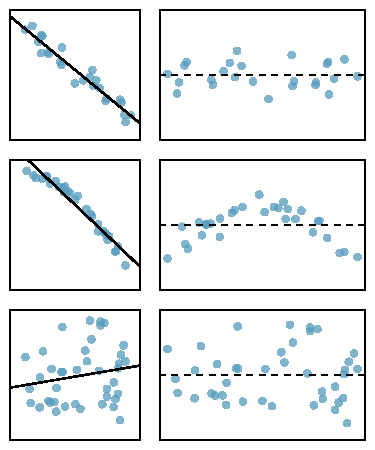
\includegraphics[width=0.6\textwidth]
{ch_simple_linear_regression_oi_biostat/figures/sampleLinesAndResPlots/sampleLinesAndResPlots.pdf}
\caption{Sample data with their best fitting lines (left) and their corresponding residual plots (right).}
\label{sampleLinesAndResPlots}
\end{figure}

Figure~\ref{prevendResidualPlot} shows a residual plot from the estimated linear model $\widehat{\text{RFFT}} = 137.55 - 1.26(\text{age})$. While the residuals show scatter around the line, there is less variability for lower predicted RFFT scores. A data analyst might still decide to use the linear model, with the knowledge that predictions of high RFFT scores may not be as accurate as for lower scores. Reading a residual plot critically can reveal weaknesses about a linear model that should be taken into account when interpreting model results. More advanced regression methods may be more suitable for these data but are beyond the scope of this text.


\begin{figure}[h]
	\centering
	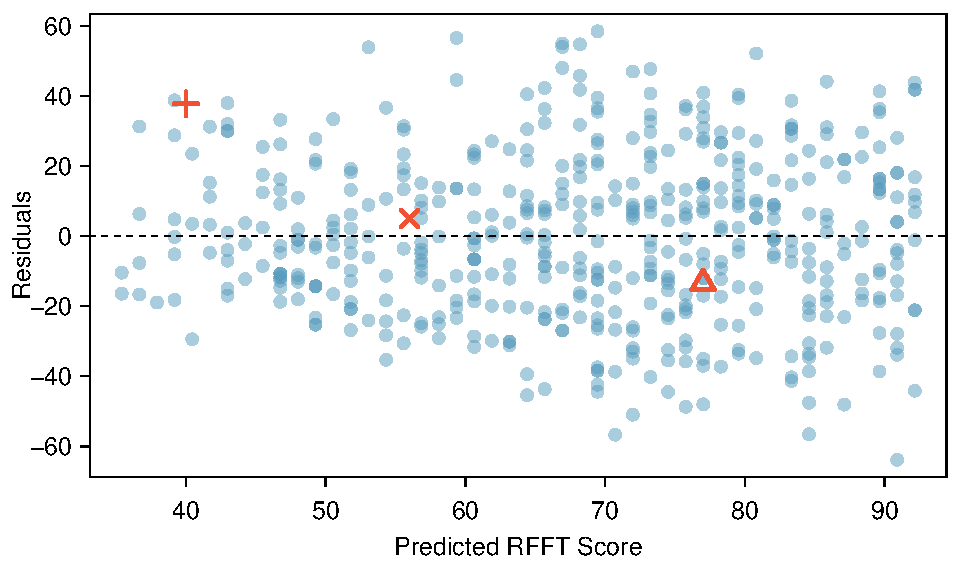
\includegraphics[width=0.8\textwidth]{ch_simple_linear_regression_oi_biostat/figures/prevendResidPlot/prevendResidPlot}
	\caption{Residual plot for the model in Figure~\ref{prevendResid}.}
	\label{prevendResidualPlot}
\end{figure}

\begin{example}{
Figure~\ref{prevendResidualPlot} shows a residual plot for the model predicting weight from height using the FAMuSS data. Assess whether the constant variability assumption holds for the linear model.
\begin{figure}[h!]
	\centering
	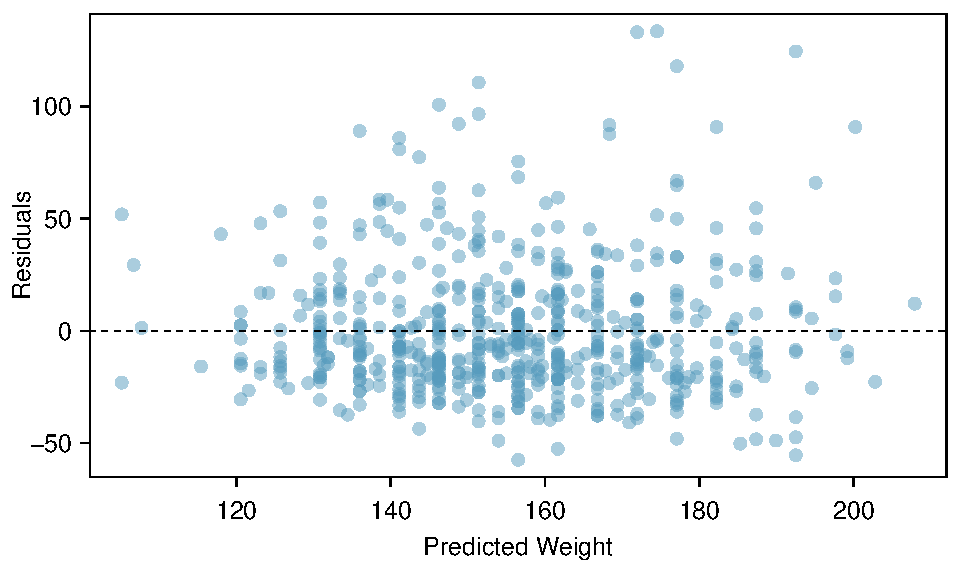
\includegraphics[width=0.6\textwidth]
	{ch_simple_linear_regression_oi_biostat/figures/famussHeightWeightResidualPlot/famussHeightWeightResidualPlot.pdf}
	\caption{A residual plot from the linear model for height versus weight in the FAMuSS data.}
	\label{famussHeightWeightResidualPlot}
	\end{figure}
}

The residuals above the line are more variable, taking on more extreme values than those below the line. Larger than expected residuals imply that there are many large weights that are under-predicted; in other words, the model is less accurate at predicting relatively large weights.
	
\end{example}

%JV: Example with log transforming the data seems misplaced here, at least without more guidance about what to do if not all assumptions are perfectly met. 


\subsubsection{Checking normality of the residuals}

\index{normal probability plot}

% check that this is indexed in chap 1 after pulling from repo

The normal probability plot, introduced in Section~\ref{assessingNormal}, is best suited for checking normality of residuals, since normality can be difficult to assess using histograms alone. Figure~\ref{prevendResidNormPlot} shows both the histogram and normal probability plot of the residuals after fitting a least squares regression to the age versus RFFT data.  
 
\begin{figure}[h!]
	\centering
	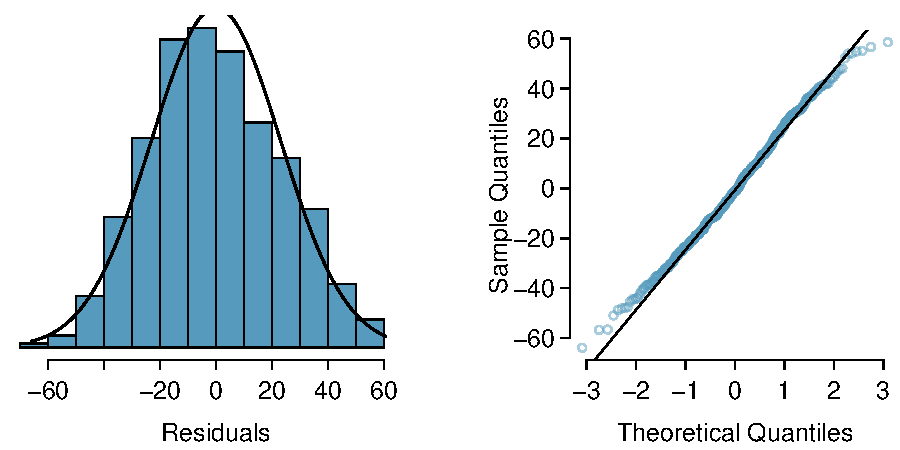
\includegraphics[width=0.8\textwidth]
	{ch_simple_linear_regression_oi_biostat/figures/prevendResidNormPlot/prevendResidNormPlot.pdf}
	\caption{A histogram and normal probability plot of the residuals from the linear model for RFFT vs. Age in the PREVEND data}
	\label{prevendResidNormPlot}
\end{figure}

The normal probability plot shows that the distribution of the residuals is very close to a normal distribution, with only a slight deviation from normality in the left and right tails.

\index{residual|)}

\subsection{Using $R^2$ to describe the strength of a fit}
\label{RSquaredLinearRegression}

\index{least squares regression!R-squared ($R^2$)|(}

The correlation coefficient $r$ measures the strength of the linear relationship between two variables. However, it is more common to measure the strength of a linear fit using $r^2$, which is commonly written as $R^2$ in the context of regression.\footnote{In software output, $R^2$ is usually labeled \termsub{R-squared}{least squares regression!R-squared ($R^2$)}.} 

The quantity $R^2$ describes the amount of variation in the response that is explained by the least squares line. While $R^2$ can be easily calculated by simply squaring the correlation coefficient, it is easier to understand the interpretation of $R^2$ by using an alternative formula (not derived here):

\[R^{2} = \dfrac{\text{variance of predicted $y$-values}}{\text{variance of observed $y$-values}}.\]
It is possible to show that $R^2$ can also be written
\[R^{2} = \dfrac{s^{2}_{y} - s_{\text{residuals}}^2}{s^{2}_{y}}.\]

In the linear model predicting RFFT scores from age, the predicted values on the least squares line are the values of RFFT that are 'explained' by the linear model. The variability of the residuals about the line represents the remaining variability after the prediction; i.e., the variability unexplained by the model. For example, if a linear model perfectly captured all the data, then the variance of the predicted $y$-values would be equal to the variance of the observed $y$-values, resulting in $R^2 = 1$. In the linear model for $\widehat{RFFT}$, the proportion of variability explained is

\[R^{2} = \dfrac{s^{2}_{RFFT} - s_{\text{residuals}}^2}{s^{2}_{RFFT}} = \dfrac{750.52 - 536.62}{536.62} = \dfrac{213.90}{750.52} = 0.285, \]
about 29\%. This is equal to the square of the correlation coefficient, $r^2 = -0.534^{2} = 0.285$. 

Since $R^2$ in simple linear regression is simply the square of the correlation coefficient between the predictor and the response, it does not add a new tool to regression.  It becomes much more  useful in models with several predictors, where it has the same interpretation as the proportion of variability explained by a model and is no no longer the square of any one of the correlation coefficients between the individual responses and the predictor.  Those models are discussed in Chapter~\ref{multipleLinearRegression}

\begin{exercise} In the FAMuSS data, the variance of \var{weight} is $1196.5$ $\text{pounds}^2$ and the variance of the residuals is 859.3. What proportion of the variability in the data is explained by the model?\footnote{About 28\%: $\frac{s_{\text{weight}}^2 - s_{\text{residuals}}^2}{s_{\text{weight}}^2} = \frac{1196.5 - 859.3}{1196.5} = \frac{337.2}{1196.5} = 0.282$}
\end{exercise}

\begin{exercise}
If a linear model has a very strong negative relationship with a correlation of -0.97, how much of the variation in the response is explained by the explanatory variable?\footnote{About $R^2 = (-0.97)^2 = 0.94$ or 94\% of the variation is explained by the linear model.}
\end{exercise}

\index{least squares regression!R-squared ($R^2$)|)}

\subsection{Categorical predictors with two levels}
\label{categoricalPredictorsWithTwoLevels}

Linear regression can be used to examine the relationship between a numerical response variable and a categorical predictor variable. This section explores the association between a country's infant mortality rate and whether or not 50\% of the population has access to adequate sanitation facilities. 

The World Development Indicators (WDI) is a database of country-level variables (i.e., indicators) recording outcomes for a variety of topics, including economics, health, mortality, fertility, and education.\footnote{http://data.worldbank.org/data-catalog/world-development-indicators}. The dataset \data{wdi.2011} contains a subset of variables on 165 countries from the year 2011.\footnote{Data collected by a Harvard undergraduate in the Statistics department.} The infant mortality rate in a country is recorded as the number of deaths in the first year of life per 1,000 live births. Access to sanitation is recorded as the percentage of the population with adequate disposal facilities for human waste. While infant mortality is measured reasonably accurately throughout the world, due to the availability of death certificates, it is more difficult to obtain precise measurements of the percentage of a population with access to adequate sanitation facilities. Instead, considering whether half the population has such access may provide a more reliable measure.  The analysis presented here is based on 163 of the 165 countries; the values for access to sanitation are missing for New Zealand and Turkmenistan.

Figure~\ref{wdiHistReg} shows that infant mortality rates are highly right-skewed, with a relatively small number of countries having high infant mortality rates. In 13 countries, infant mortality rates are higher than 70 deaths per thousand live births. Figure~\ref{wdiHistLog} shows infant mortality after a log transformation; the following analysis will use the more nearly symmetric transformed version of \var{inf.mortality}.  The least squares regression line has the form
\begin{align}
    \widehat{\log(\texttt{inf.mortality)}} = b_0 + b_1 \times \texttt{sanit.access},
	\label{logInfMortalitySanitRegress}
\end{align}
where \texttt{sanit.access} = 1 if  at least 50\% of the population has access to adequate sanitation (high access) and 0 otherwise (low access).

\begin{figure}[ht]
	\centering
	\subfigure[]{
		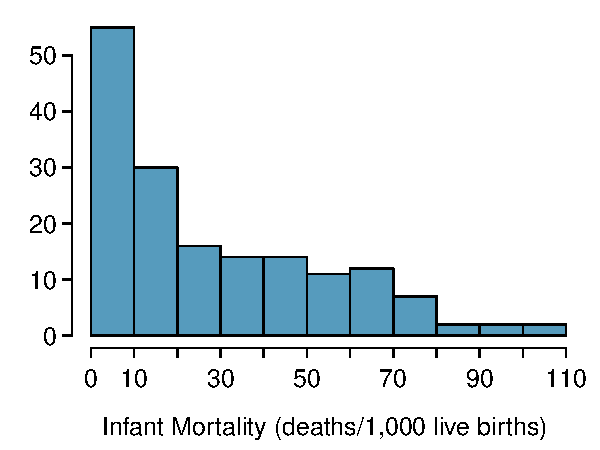
\includegraphics[width=0.46\textwidth]
		{ch_simple_linear_regression_oi_biostat/figures/wdiHistTransform/wdiHistReg}
		\label{wdiHistReg}
	}
	\subfigure[]{
		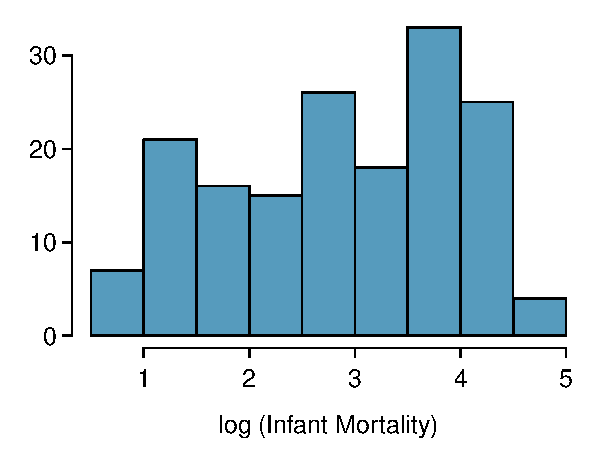
\includegraphics[width=0.46\textwidth]
		{ch_simple_linear_regression_oi_biostat/figures/wdiHistTransform/wdiHistLog}
		\label{wdiHistLog}
	}
	\caption{\subref{wdiHistReg} Histogram of infant mortality, measured in deaths per 1,000 live births in the first year of life. \subref{wdiHistLog} Histogram of the log-transformed infant mortality.}
	\label{wdiHistTransform}
\end{figure}


Figure~\ref{wdiPlot} shows a scatterplot of \texttt{log(\text{inf.mortality})} against the categorical variable for sanitation access, coded \texttt{1} if at least 50\% of the population has access to adequate sanitation, and \texttt{0} otherwise\footnote{There are no recorded values for access to sanitation for New Zealand and Turkmenistan, and those countries have been dropped from the scatterplot}. Since there are only two values of the predictor, the values of infant mortality are stacked above the two predictor values 0 and 1. The estimated least squares regression line has intercept and slope and parameters of 4.018 and -1.681, respectively. While the scatterplot appears unlike those in previous contexts, the interpretation of the parameters remains unchanged; -1.681 is the change in the log of infant mortality when the categorical predictor changes from low access to sanitation facilities to high access. The intercept term 4.018 is the estimated log infant mortality for the set of countries where less than 50\% of the population has access to adequate sanitation facilities (\var{sanit.access} = 0).

\begin{figure}[h]
	\centering
	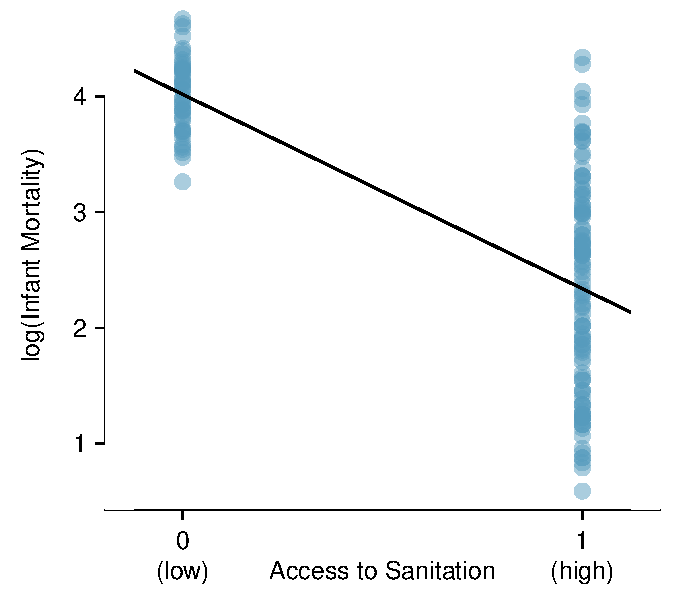
\includegraphics[width=0.6\textwidth]{ch_simple_linear_regression_oi_biostat/figures/wdiPlot/wdiPlotB}
	\caption{Country-level infant mortality rates, divided into low access ($x=0$) and high access ($x=1$) to sanitation. The least squares regression line is also shown.}
	\label{wdiPlot}
\end{figure}

%JV: Change the name of the plot to wdiPlotA to see a version of the plot that is closer to base R. OI code uses dotplot instead of plot to suppress the tick mark labeling on the x-axis and more easily add labels.

In addition to inducing symmetry in the response variable \var{inf.mortality}, the log transformation provides another, more natural way to examine the association. Using the model in Equation~\ref{logInfMortalitySanitRegress}, the prediction equation can be written
\[
    \widehat{\log(\texttt{inf.mortality)}} = 4.018 -1.681 \times \texttt{sanit.access}.
\]
Exponentiating both sides of the equation yields
\[
    \widehat{\texttt{inf.mortality}} = e^{4.018}e^{-1.681 \times \texttt{sanit.access}}.
\]
When \var{sanit.access} = 0, the equation simplifies to $\exp(4.018) = 55.590$ deaths among 1,000 live births; this is the estimated infant mortality rate in the countries with low access to sanitation facilities.  When \var{sanit.access} = 1, the estimated infant mortality rate is $(55.590)(\exp(-1.681))= (55.590)(0.186)$ deaths per 1,000 live births.  The infant mortality rate drops by a factor of 0.186. The rate in the high access countries is approximately 20\% of that in the low access countries, a drop of 80\%. When examining event rates in public health, associations are typically measured using rate ratios rather than rate differences.


\begin{example}{Check the assumptions of constant variability around the regression line and normality of the residuals in the model for the relationship between the transformed infant mortality variable and access to sanitation variable. Residual plots are shown in Figure~\ref{wdiResid}.
		
\begin{figure}[h]
	\centering
	\subfigure[]{
		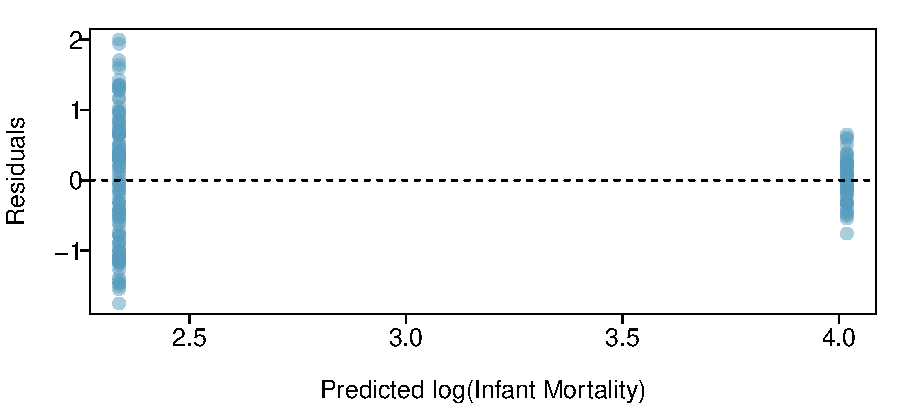
\includegraphics[width=0.45\textwidth]
		{ch_simple_linear_regression_oi_biostat/figures/wdiResid/wdiResidualPlot}
		\label{wdiResidPlot}
	}
	\subfigure[]{
		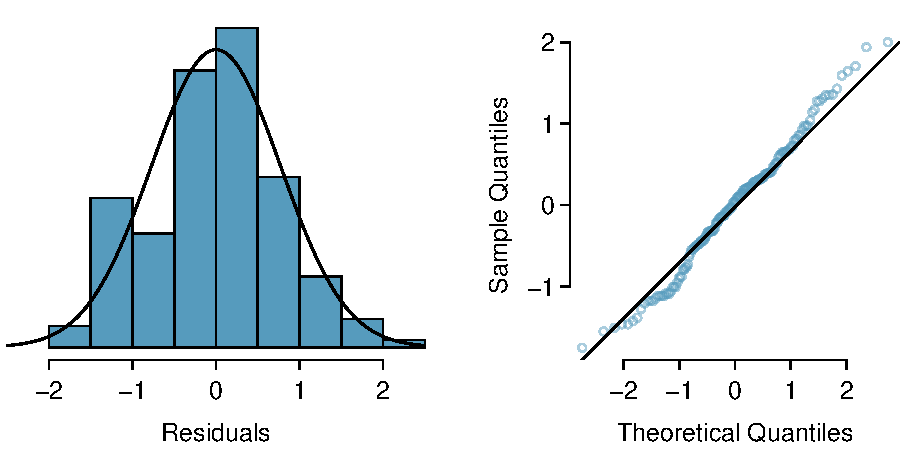
\includegraphics[width=0.45\textwidth]
		{ch_simple_linear_regression_oi_biostat/figures/wdiResid/wdiResidNormPlot}
		\label{wdiResidNormPlot}
	}
	\caption{\subref{wdiResidPlot} Residual plot of \texttt{log(inf.mortality)} and \texttt{sanit.access}. \subref{wdiHistLog} Histogram and normal probability plot of the residuals.}
	\label{wdiResid}
\end{figure}		
}		

While the normal probability plot does show that the residuals are approximately normally distributed, the residual plot reveals that variability is far from constant around the two predictors. Another method for assessing the relationship between the two groups is advisable; this is discussed further in Section~\ref{categoricalTwoGroup}.

% this ref does not get expanded as subsection number
\label{wdiAssumptionsEx}	

\end{example}


\subsection{Outliers in regression}

Depending on their position, data points in a scatterplot have varying degrees of contribution to the estimated parameters of a regression line. Points that are at particularly low or high values of the predictor ($x$) variable are said to have \term{high leverage}, since they have a large influence on the estimated intercept and slope of the regression line; observations with $x$ values closer to the center of the distribution of $x$ do not have a large effect on the slope. 

A data point in a scatterplot is considered an \term{outlier in regression} if its value for the response ($y$) variable does not follow the general linear trend in the data. Outliers that sit at extreme values of the predictor variable (i.e., have high leverage) have the potential to contribute disproportionately to the estimated parameters of a regression line. If an observation does have a strong effect on the estimates of the line, such that estimates change substantially when the point is omitted, the observation is \term{influential}. These terms are formally defined in advanced regression courses.


This section examines the relationship between infant mortality and number of doctors, with data for each state and the District of Columbia. Infant mortality is the number of infant deaths in the first year of life per 1,000 live births, and the number of doctors is coded as number of doctors per 100,000 members of the population. Figure~\ref{infMortUS} shows scatter plots with infant mortality on the $y$-axis and number of doctors per 100,000 members of the population on the $x$-axis.\footnote{Data are from the Statistical Abstract of the United States, published by the US Census Bureau. Data are for 2010.} 

One point in Figure~\ref{infMortUSDC}, marked in red, is clearly distant from the main cluster of points. This point corresponds to the District of Columbia, where there were approximately 807.2 doctors per 100,000 members of the population, and the infant mortality rate was 11.3 per 1,000 live births; it is both an outlier and an observation with high leverage. Figure~\ref{infMortUSnoDC} illustrates that the DC observation is influential. Not only does the observation simply change the numerical value of the slope parameter, it reverses the direction of the linear trend; the regression line fitted with the complete dataset has a positive slope, but the line re-fitted without the DC observation has a negative slope. The large number of doctors per population is due to the presence of several large medical centers in an area with a population that is much smaller than a typical state.

\begin{figure}[h!]
	\centering
	\subfigure[]{
		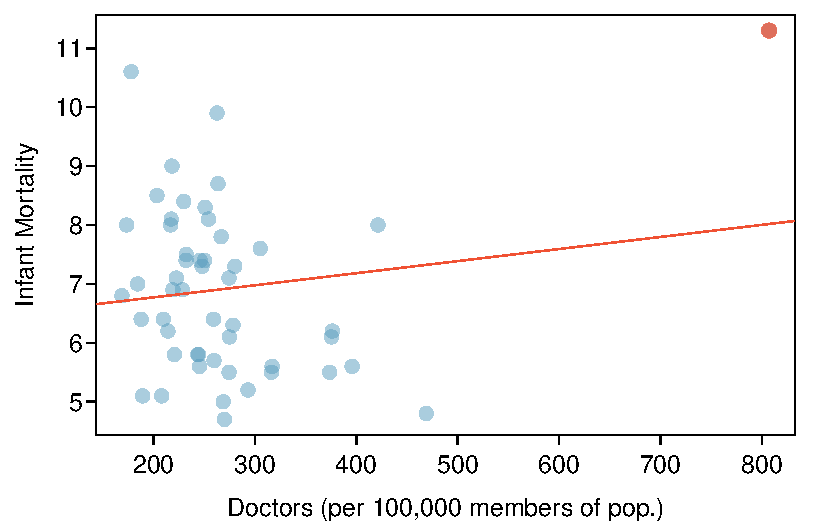
\includegraphics[width=0.65\textwidth]
		{ch_simple_linear_regression_oi_biostat/figures/infMortUS/infMortUS}
		\label{infMortUSDC}
	}
	\subfigure[]{
		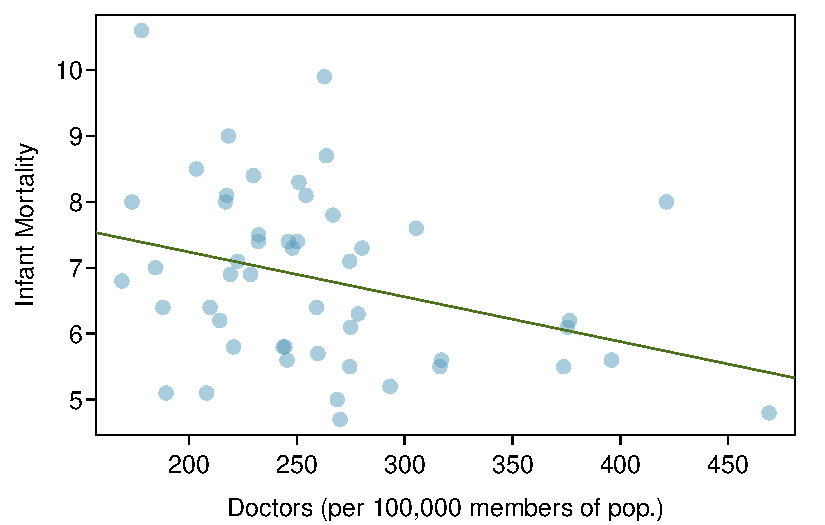
\includegraphics[width=0.65\textwidth]
		{ch_simple_linear_regression_oi_biostat/figures/infMortUS/infMortUSnoDC}
		\label{infMortUSnoDC}
	}
	\caption{\subref{infMortUS} Plot including District of Columbia data point. \subref{infMortUSnoDC} Plot without influential District of Columbia data point.}
	\label{infMortUS}
\end{figure}	

It might seem natural to ask whether or not an influential point should be removed from a dataset before a regression line is fitted, but that may not be the right question. Instead, it is usually more important to question whether the influential point might be an error in the data, or whether it belongs in the dataset. In this case, the District of Columbia has many special characteristics that may make comparisons with other states inappropriate. 

Generally speaking, if an influential point arises from random sampling from a large population and is not a data error, it should be left in the dataset, since it probably represents a small subset of the population from which the data were sampled. 

\begin{exercise}Once the influential DC point is removed, assess whether it is appropriate to use linear regression on these data by checking the four assumptions behind least squares regression: linearity of the association, constant variability in the scatter about the line, independent observations, and approximate normality of the residuals.\footnote{The scatter plot in Figure~\ref{infMortUSnoDC} does not show any nonlinear trends. Similarly, Figure~\ref{infMortUSResidualPlot} does not indicate any nonlinear trends or noticeable difference in the variability of the residuals, although it does show that there are relatively few observations for low values of predicted infant mortality. From Figure~\ref{infMortUSResidNormPlot}, the residuals are approximately normally distributed. Infant mortality across the states reflects a complex mix of different levels of income, access to health care, and individual state initiatives in health care; these and other state-specific features probably act independently across the states, although there is some dependence from federal influence such as funding for pre-natal care. Overall, independence seems like a reasonable assumption.} 

\begin{figure}[h]
	\centering
	\subfigure[]{
		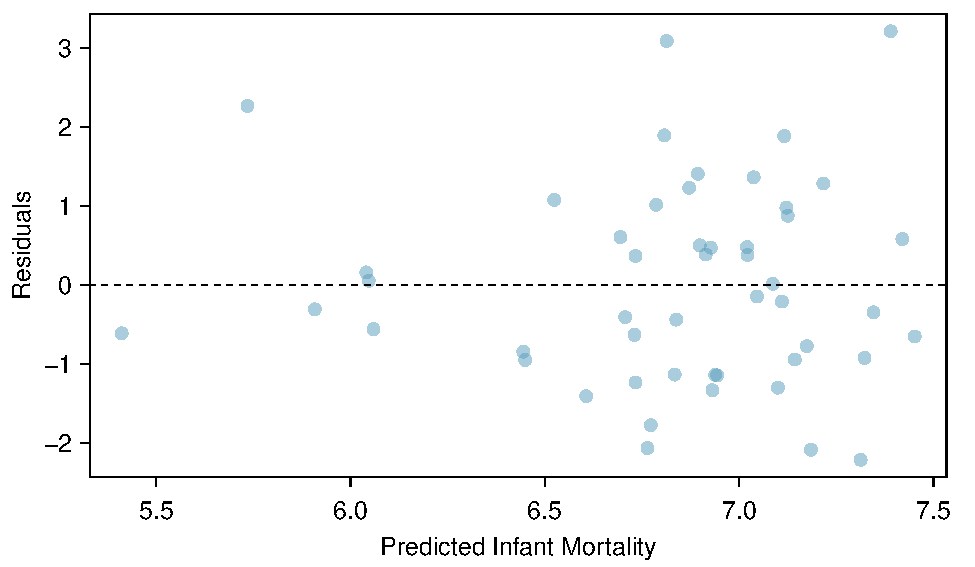
\includegraphics[width=0.45\textwidth]
		{ch_simple_linear_regression_oi_biostat/figures/infMortUSResid/infMortUSResidualPlot.pdf}
		\label{infMortUSResidualPlot}
	}
	\subfigure[]{
		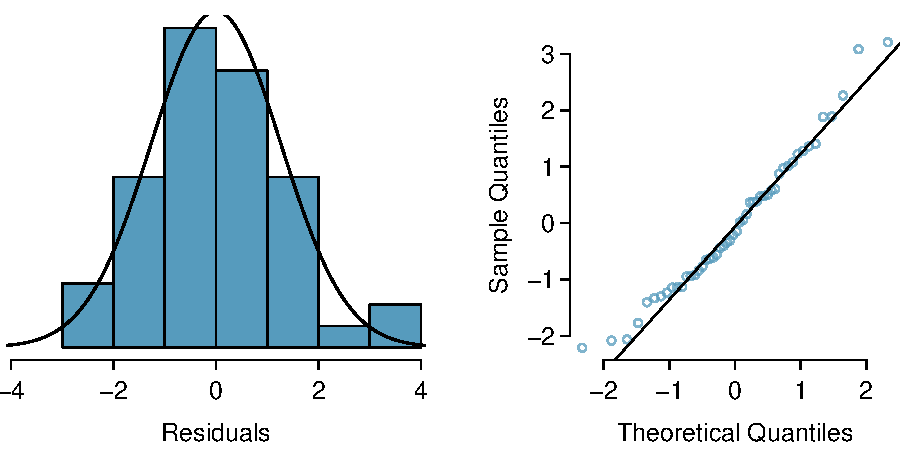
\includegraphics[width=0.45\textwidth]
		{ch_simple_linear_regression_oi_biostat/figures/infMortUSResid/infMortUSResidNormPlot.pdf}
		\label{infMortUSResidNormPlot}
	}
	\caption{\subref{infMortUSResidualPlot} Residual plot of \texttt{inf.mortality} and \texttt{doctors}. \subref{infMortUSResidNormPlot} Histogram and normal probability plot of the residuals.}
	\label{infMortUSResid}
\end{figure}

\label{exampleInfantMortalityAssumptions}
\end{exercise}

It is important to be especially careful about outliers when predictors are categorical variables.  Figure~\ref{wdiPlot} shows the regression line passing through the mean response variable for each of the two categories \var{sanit.access} = 1 and \var{sanit.access} = 0. It is generally true that when a categorical predictor variable has two levels, the regression line passes through the mean of each group. If one group is particularly small and has a very different set of values for the response variable, that category will have large influence on the estimated slope.

\section{Statistical inference with regression}
\label{inferenceRegression}

The previous sections in this chapter have focused on linear regression as a tool for summarizing trends in data and making predictions. These numerical summaries are analogous to the methods discussed in Chapter~\ref{introductionToData} for displaying and summarizing data. However, regression is also used in making inferences about a population. 

The same ideas covered in Chapters~\ref{foundationsForInference} and \ref{inferenceForNumericalData} about using data from a sample to draw inferences about population parameters apply with regression, but the population model is more complex. The basis for inference in regression relies on the population linear model for the relationship between an explanatory variable $X$ and a response variable $Y$ given by
\begin{align}
Y = \beta_0 + \beta_1 X + \varepsilon,
\label{regressionPopulationModel}
\end{align}
where $\epsilon$ is assumed to have a normal distribution with mean 0 and standard deviation $\sigma$ ($\varepsilon \sim N(0, \sigma)$).  In words, this population model specifies that a response $Y$ has value $\beta_0 + \beta_1 X$ plus a random term that pushes $Y$ symmetrically above or below its value on the line. Since $E(\varepsilon) = 0$, this model can also be written as $Y\sim N(\mu_x)$, with $ \mu_x = E(Y) = \beta_0 + \beta_1 X$.  The term $\varepsilon$ is the population model for the observed residuals $e_i$ in regression. 

The set of ordered pairs $(x_i,y_i)$ used when fitting a least squares regression line are assumed to have been sampled from a population in which the relationship between the explanatory and response variables is given by Equation~\ref{regressionPopulationModel}. Under this assumption, the slope and intercept values of the least squares regression line, $b_0$ and $b_1$, are estimates of the population parameters $\beta_0$ and $\beta_1$; $b_0$ and $b_1$ have sampling distributions, just as $\overline{X}$ does when thought of as an estimate of a population mean $\mu$. A more advanced treatment of regression would demonstrate that the sampling distribution of $b_1$ is normal with mean $E(b_1) = \beta_1$ and standard deviation
\begin{align*}
  \sigma_{b_1} = \frac{\sigma}{\sqrt{\sum(x_i -\overline{x})^2}}
\end{align*}. 
The sampling distribution of $b_0$ has mean $E(b_0) = \beta_0$ and standard deviation 
\begin{align*}
  \sigma_{b_0} = \sigma \sqrt{\frac{1}{n} + \frac{\overline{x}^2}{\sum(x_i - \overline{x})^2}}.
\end{align*} 
In both of these expressions, $\sigma$ is the standard deviation of $\varepsilon$.

Hypothesis tests and confidence intervals for regression parameters have the same basic form as tests and intervals about population means. Inference is usually done about the slope; inference about the intercept term is rare, and limited to the few problems where the vertical intercept has scientific meaning. \footnote{In some applications of regression, the predictor $x$ is replaced by $x^* = x - \overline{x}$.  In that case, the vertical intercept is the value of the line when $x^* = 0$, or $x = \overline{x}$.}

The test statistic for a null hypothesis $H_0: \beta_1 = \beta^0_1$ about a slope parameter is
\[t = \frac{b_1 - \beta^0_1}{s.e.(b_1)},\]
where the formula for $s.e.(b_1)$ is given below.
In this setting, $t$ has a $t$-distribution with $n - 2$ degrees of freedom, where $n$ is the number of ordered pairs used to calculated the least squares line.  

Typically, hypothesis testing in regression involves tests of whether the $x$ and $y$ variables are associated; in other words, whether the slope is significantly different from 0. In these settings, the null hypothesis is that there is no association between the explanatory and response variables, or $H_0: \beta_1 = 0 = \beta^0_1$, in which case
\[t = \frac{b_1}{s.e.(b_1)}.\]
The hypothesis is rejected in favor of the two-sided alternative $H_A: \beta_1 \neq 0$ with significance level $\alpha$ when $|t| \ge t^*_{n - 2}$, where $t^*_{n - 2}$ is the point on a $t$-distribution with $n-2$ degrees of freedom that has $\alpha/2$ area to its right.

A two-sided confidence interval for $\beta_1$ is given by 
\[b_1 \pm s.e.(b_1)t^*_{n-2}.\]
Tests for one-sided alternatives and one-sided confidence intervals make the usual adjustments to the rejection rule and confidence interval, and $p$-values are interpreted just as in Chapters 4 and 5.

\subsubsection{Formulas for calculating standard errors}

Statistical software is typically used to obtain $t$-statistics and $p$-values for inference with regression, since using the formulas for calculating standard error can be cumbersome.

The standard errors of $\beta_0$ and $\beta_1$ used in confidence intervals and hypothesis tests replace $\sigma$ with $s$, the standard deviation of the residuals from a fitted line. Formally, 
\begin{align*}
e_{i} &= \textrm{observed response - predicted response}\\
&= y_{i}-\hat{y}_{i}\\
&= y_{i}-b_{0}-b_{1}x_{i}, \text{   and} \\
s &= \sqrt{\frac{\Sigma e^{2}_{i}}{n-2}} =  \sqrt{\frac{\Sigma (y_{i}-\hat{y}_{i})^{2}}{n-2}}.
\end{align*}
The two standard errors are
\begin{align*}
\text{s.e.}_{b_1} &= \frac{s}{\sqrt{\sum(x_i -\overline{x})^2}} \text{   and}\\
\text{s.e.}_{b_0} &= s \sqrt{\frac{1}{n} + \frac{\overline{x}^2}
	{\sum(x_i - \overline{x})^2}}.
\end{align*}

\begin{example}{Is the number of doctors per 100,000 members of the population in a state significantly associated with infant mortality rate? Let $\alpha = 0.05$. }
	
The question implies that the District of Columbia should not be included in the analysis. The assumptions for applying a least squares regression have been verified in Exercise~\ref{exampleInfantMortalityAssumptions}. Whenever possible, formal inference should be preceded by a check of the assumptions for regression.

The null and alternative hypotheses are $H_0:\beta_1 = 0$ and $H_A:\beta_1 \neq 0.$	

The numerical output from the analysis that \textsf{R} returns is shown in Table~\ref{infantMortalityInferenceOutput}.\footnote{Other software packages, such as Stata or Minitab, provide similar information but with slightly different labeling.} 

\begin{table}[ht]
	\centering
	\begin{tabular}{rrrrr}
		\hline
		& Estimate & Std. Error & t value & Pr($>$$|$t$|$) \\ 
		\hline
		(Intercept) & 8.5991 & 0.7603 & 11.31 & 0.0000 \\ 
		Doctors Per 100,000 & -0.0068 & 0.0028 & -2.40 & 0.0206 \\ 
		\hline
	\end{tabular}
	\caption{Regression of doctors per 100,000 vs infant mortality for the 50 US states in 2010}
	\label{infantMortalityInferenceOutput}
\end{table}

% xtable(lm(us.infant.mortality.2011$infant.mortality[a] ~us.infant.mortality.2011$doctors.per.100000[a]))
% latex table generated in R 3.2.3 by xtable 1.8-0 package
% Tue Oct 25 11:49:28 2016
% variable names have  been edited

Using either the formulas or the \textsf{R} output, the estimated slope of the least squares line is -0.0068, with standard error 0.0028. The $t$-statistic equals -2.40, and the probability that the absolute value of a $t$-statistic with $50-2=48$ degrees of freedom is smaller than  $-2.40$ or larger than $2.40$ is 0.021. Since $p = 0.021 < 0.05$, the data support the alternative hypothesis that the number of physicians is associated with infant mortality; the sign of the slope implies that the association is negative.  States with more doctors tend to have lower rates of infant mortality.

It is incorrect to make claims of causality from these data, such as stating that an additional 100 physicians (per 100,000 residents) would lead to a decrease of 0.68 in the infant mortality rate. Additionally, the R-squared statistic is 0.107, so the model explains only about 10\% of the state-to-state variability in infant mortality; there are many other factors affecting infant mortality that are not accounted for in the model.\footnote{$R^2$ given in additional \textsf{R} output not shown here.}
One important implicit assumption being made in this example is that data from the year 2010 are representative; in other words, that the relationship between number of physicians and infant mortality is constant over time. 
\label{exampleInfantMortalityInference}		
\end{example}

\begin{exercise} Construct a 95\% two-sided confidence interval for the slope $\beta_{1}$ in the state-level infant mortality data.\footnote{The $t^{\star}$ value for a $t$-distribution with 48 degrees of freedom is 2.01, and the standard error of $b_1$ is 0.0028. The 95\% confidence interval is $-0.0068 \pm 2.01(0.0028)$ = (-0.0124, -0.0012). } 
\end{exercise}

\subsubsection{Connection to two-group hypothesis testing}
\label{categoricalTwoGroup}

Conducting a regression analysis with a numerical response variable and a categorical predictor with two levels is analogous to conducting a two-group hypothesis test. For example, Section~\ref{categoricalPredictorsWithTwoLevels} shows a regression model that compares the average infant mortality rate in countries with low access to sanitation facilities versus high access.\footnote{Recall that a log transformation was used on the infant mortality rate.} The intercept parameter $b_0$ is the average predicted log(mortality rate) (4.018) in countries where 50\% or less of the population has adequate access to sanitation facilities. The slope parameter $b_1$ (-1.681) is the difference between the means of the log(mortality rate) in the low access group and the high access group, with the negative sign indicating that the log(mortality rate) in the high access group is lower. Recall that in this example, the estimated infant mortality rate in the low access group is $\exp(4.018) = 55.5898$ deaths per 1,000 live births and the rate in the high access group is estimated to be $\exp(-1.1681) = 0.186$ times that rate.

The connection between regression and hypothesis testing also extends to inference. When the pooled standard deviation assumption (Section~\ref{pooledStandardDeviations}) is used, the $t$-statistic and $p$-values from a hypothesis test are equivalent to those returned from a regression model. 

Here is the \textsf{R} output from a regression model in which `High Access' is coded 1 for the countries where at least 50\% of the population has access to adequate sanitation and 0 otherwise:


\begin{table}[ht]
\centering
\begin{tabular}{rrrrr}
  \hline
 & Estimate & Std. Error & t value & Pr($>$$|$t$|$) \\ 
  \hline
(Intercept) & 4.0184 & 0.1100 & 36.52 & < 0.001 \\ 
  High Access & -1.6806 & 0.1322 & -12.72 & 0.001 \\ 
   \hline
\end{tabular}
\caption{Regression of log(infant mortality) versus sanitation access} 
\label{regressLogInfMortAccess}
\end{table}

%predictor name changed
%access.log.inf.mort.regress = lm(log(wdi.2011$inf.mort) ~wdi.2011$sanit.access.factor)
%xtable(access.log.inf.mort.regress, caption = "Regression of log(infant mortality) versus sanitation access", label = "regressLogInfMortAccess")

% latex table generated in R 3.3.2 by xtable 1.8-2 package
% Sun Nov 26 14:50:15 2017

The abbreviated \textsf{R} output from a $t$-test that assumes equal standard deviations is shown in Table~\ref{tTestSanitEqualStd}.  One hundred sixty-three countries are represented in the dataset, 50 and 113 in the low and high access categories, respectively,  so the degrees of freedom in the pooled test has value 161.  The $t$-statistic has value 12.72, while the $t$-value in the regression is -12.72, so the two-sided $p$-value is the same small number.   The difference in sign arises from the coding; in the $t$-test output, the mean of log(infant mortality) in the high access group was subtracted from the mean in the low access group.  In the regression model, the negative sign reflects the reduction in log(infant mortality) in changing from low access to high access countries.


\begin{table}[ht]
\centering
\begin{tabular}{rll}
  \hline
 & Test & Results \\ 
  \hline
1 &  Two Sample t-test: & t(161) = 12.72, p $<$ .001 \\ 
   \hline
\end{tabular}
\caption{T-test assuming equal st.dev} 
\label{tTestSanitEqualStd}
\end{table}

%equal.var.t.test <- t.test(log(wdi.2011$inf.mort) ~  wdi.2011$sanit.access.factor, var.equal = T)
%xtable(t_out(toutput=equal.var.t.test, d.corr = FALSE, print = TRUE),caption = "T-test assuming equal st.dev",label = "tTestSanitEqualStd")
% latex table generated in R 3.3.2 by xtable 1.8-2 package
% Sun Nov 26 14:56:30 2017
% dh edited the p-value in the regression output to match <0.001 in t-test.


Example~\ref{wdiAssumptionsEx} showed that the constant variability assumption does not hold for these data. Instead, a researcher interested in comparing the infant mortality rates between these two groups might choose to conduct a two-group hypothesis test without using the pooled standard deviation assumption, shown in Table~\ref{tTestSanitUnEqualStd}\footnote{The version of the $t$-test that does not assume equal standard deviations and uses non-integer degrees of freedom is often called the Welch test}. This changes the $t$-statistic and degrees of freedom, but in this case does not have a noticeable effect on the $p$-value.

\begin{table}[ht]
\centering
\begin{tabular}{rll}
  \hline
 & Test & Results \\ 
  \hline
1 & Welch Two Sample t-test: & t(155.82) = 17.36, p $<$ .001 \\ 
   \hline
\end{tabular}
\caption{T-test assuming unequal st.dev} 
\label{tTestSanitUnEqualStd}
\end{table}
%unequal.var.t.test <- t.test(log(wdi.2011$inf.mort) ~  wdi.2011$sanit.access.factor)
%xtable(t_out(toutput=unequal.var.t.test, d.corr = FALSE, print = TRUE))
% latex table generated in R 3.3.2 by xtable 1.8-2 package
% Sun Nov 26 14:58:35 2017


\section{Notes}

This chapter provides only a brief introduction to simple linear regression.   In more advanced courses substantial portions of the course material or the text are devoted to the details and subtleties of fitting straight line models. For instance,  there are strategies for adjusting an analysis when one or more of the assumptions outlined in this chapter do not hold. There are methods to assess numerically the leverage or influence that each case has on the fit, not just the obvious outliers.  The goal of this chapter is to introduce enough of the principles of simple regression to so the topic can serve as a foundation for the more useful and commonly used regression models with more than one predictor examined in Chapter~\ref{multipleLinearRegression}.  Nevertheless, there are some important things to keep in mind when fitting straight lines to data.

\begin{itemize}

\item When fitting a simple linear regression, make a scatter plot with a least squares line, even when the predictor is a categorical variable with two levels.  Nonlinear trends or outliers are often obvious in scatter plots.  If outliers are evident, the source of the data should when possible, since outliers result from errors in data collection.  If there has not been an error or the data collection process is not accessible, consider whether the outlier does not belong to the target population of inference, such as the District of Columbia in the data on infant mortality shown in Figure~\ref{infMortUS}.
 
   \item  There a several variants of the residual plots used for diagnostic and show in Section~\ref{checkingResiduals}.  The plots used here which plot the predicted values along the horizontal axis easily generalize to settings with multiple predictors examined in Chapter~\ref{MultipleLinearRegression}, since there is always a single predicted value even when there is more than one predictor.  If the only model used is a simple linear regression, plotting residuals on the vertical axis against the value of the predictor on the horizontal axis may make it easier to identify a case with a notable residual.  Data analysts will sometimes plot residuals against the case number of the predictor since runs of large or small residuals may indicate adjacent cases that are correlated.

   \item  The $R^2$ statistic is widely used in the social sciences where the unexplained variability in the data is typically much larger than the variability captured or explained by a model.  The $R^2$ statistic is a useful reminder that a regression coefficient can be highly statistically significant even with a low proportion of explained variability.  The $R^2$ should not be interpreted as a measure of the quality of the fit of the model.  Is it possible for $R^2$ to be large even when the data do not show a linear relationship. It is important to be aware of what information $R^2$ does and does not provide.

   \item Inference with regression models is more subtle than it may appear, and the difficulties are rarely with the formulas for the test statistics or standard errors.  Linear regression models are often estimated after an investigator has noticed a linear relationship in a dataset that can be represented by a straight line, and experienced investigators can often guess correctly that regression coefficients will be statistically significant before calculating a $p$-value.  This is different than the situation described in Chapter~\ref{foundationsForInference}, where the correctness of the probability of a type I error depends on the null hypothesis being specified in advance, usually when a study is designed.  There are situations where an intended regression model is specified in advance, but they are relatively rare, at least compared to two-sample tests.  But regression models are important tools and should not be abandoned because of this issue.  It is better to always be a bit skeptical about a small $p$-value in a regression setting and to be aware that it is safer to see if a statistically significant relationship in a regression model can be confirmed in an independent, validation dataset.  Advanced courses often discuss this issue at length.

  \end{itemize}

